% filename: chap-results-v4.tex
\chapter{Results and Analysis}
\label{chap:results}
\setlength{\emergencystretch}{1.5em}

% ============================================================
\section{Experimental Overview}
\label{sec:results_overview}
% ============================================================

This chapter presents the experimental results of the Energy-Aware
Telecom Tower Management study and evaluates the three pre-registered
hypotheses introduced in Chapter~\ref{chap:problem}.  The consolidated
results file contained 11{,}340 rows; after removing 1{,}800 exact
duplicate rows associated with policy~A6, the final analysis dataset
comprised 9{,}540 unique episode records.

The evaluation campaign consisted of two parts
(Table~\ref{tab:exp_scope}).  The \emph{full-coverage evaluation}
assessed RLInv, B0, B1, TrackB, and A6 across all ten ITU/Zindi sites
under both normal ($\mu=24$\,h) and delayed ($\mu=48$\,h) logistics
scenarios.  The \emph{targeted ablation evaluation} assessed A5 (no
inventory observation) on the two constrained sites under both logistics
scenarios, and A7 (no action masking) on the same constrained sites
under the normal scenario only.  The evaluation is therefore not a
fully balanced $7 \times 10 \times 2$ factorial design; coverage is
policy-specific and is documented in Table~\ref{tab:exp_scope}.

\begin{table}[htb]
\centering
\small
\caption{Evaluation campaign scope.  Coverage is policy-specific;
see notes column for A5 and A7 restrictions.}
\label{tab:exp_scope}
\begin{tabular}{lrl}
\toprule
\textbf{Item} & \textbf{Value} & \textbf{Notes} \\
\midrule
Unique episode records   & 9{,}540  & After removing 1{,}800 duplicate rows \\
Seeds per policy         & 3        & Seeds 42, 123, 777 \\
Episodes per seed        & 30       & 15-day test window \\
\midrule
\multicolumn{3}{l}{\textit{Full-coverage policies (all 10 sites, normal + delayed):}} \\
\quad RLInv, B0, B1, TrackB, A6 & 5 policies & 10 sites $\times$ 2 scenarios $\times$ 3 seeds \\
\multicolumn{3}{l}{\textit{Targeted ablation policies:}} \\
\quad A5 (no inventory obs.) & site5, site10 & Normal + delayed scenarios \\
\quad A7 (no action masking) & site5, site10 & Normal scenario only \\
\midrule
Primary metric           & EENS     & kWh per episode \\
Statistical unit         & Seed-level mean & $n=3$ \\
\bottomrule
\end{tabular}
\end{table}

The primary analysis focuses on constrained sites (site~5 and site~10)
where outage frequency, load magnitude, and limited battery autonomy
create conditions under which inventory management decisions materially
affect reliability outcomes.  Cross-site results covering all ten sites
are presented in Section~\ref{sec:cross_site}.  All results in
Sections~\ref{sec:reliability}--\ref{sec:ablation} use the normal
logistics scenario unless otherwise stated; the delayed scenario is
examined in Section~\ref{sec:delayed}.


% ============================================================
\section{Reliability Performance}
\label{sec:reliability}
% ============================================================

\subsection{Main result: policy comparison on constrained sites}

Table~\ref{tab:main_results} reports the primary reliability metrics for
all seven policies on constrained sites under the normal logistics
scenario.

\begin{table}[htb]
\centering
\small
\caption{Policy comparison on constrained sites (site~5, site~10),
normal logistics scenario.  Values are seed-level means ($n=3$);
Std is the between-seed standard deviation.  Policies ranked by
mean EENS.}
\label{tab:main_results}
\begin{tabular}{llrrrr}
\toprule
\textbf{Rank} & \textbf{Policy} & \textbf{EENS (kWh)}
    & \textbf{Std} & \textbf{Uptime (\%)} & \textbf{Category} \\
\midrule
1 & RLInv (proposed)    & \textbf{488.5} &  92.4 & \textbf{88.6} & Proposed \\
2 & B1 (reorder rule)   &          546.4 &  28.8 &          87.2 & Baseline \\
3 & A5 (no inv.\ obs.)  &          564.5 & 116.8 &          86.3 & Ablation \\
4 & A7 (no masking)     &          648.2 & 358.9 &          86.5 & Ablation \\
5= & TrackB (hier.\ RL)  &          730.9 &  14.0 &          83.0 & Ablation \\
5= & A6 (fixed $(s,S)$)  &          730.9 &  14.0 &          83.0 & Ablation \\
7 & B0 (threshold rule) &          971.1 &   4.4 &          77.3 & Baseline \\
\bottomrule
\end{tabular}
\end{table}

RLInv achieves the lowest mean EENS (488.5\,kWh) and highest uptime
(88.6\%) among all policies.  Relative to RLInv, comparator EENS is
49.6\% higher for both TrackB and the fixed-ordering ablation A6
(both 730.9\,kWh), 11.9\% higher for B1 (546.4\,kWh), and 98.8\%
higher for B0 (971.1\,kWh).  These values are reported as
\emph{comparator EENS excess over RLInv}, computed as
$(\text{Comparator} - \text{RLInv})/\text{RLInv} \times 100\%$;
positive values favour RLInv.

A structural observation is that no hard feasibility violations were
recorded in any rollout under the normal constrained-site evaluation,
as summarised in Table~\ref{tab:violations}.  Performance differences
therefore arise from differences in reliability and diesel-allocation
quality rather than from overt infeasibility.

\begin{table}[htb]
\centering
\small
\caption{Hard feasibility violations and stockout events in the normal
constrained-site evaluation (site~5 and site~10, all seeds combined).}
\label{tab:violations}
\begin{tabular}{lrr}
\toprule
\textbf{Policy} & \textbf{Hard violations} & \textbf{Stockout events} \\
\midrule
RLInv   & 0 & 0 \\
B0      & 0 & 0 \\
B1      & 0 & 0 \\
TrackB  & 0 & 0 \\
A6      & 0 & 0 \\
A5      & 0 & 0 \\
A7      & 0 & 0 \\
\bottomrule
\end{tabular}
\end{table}

\subsection{Pairwise statistical comparison}

Figure~\ref{fig:eens_comparison} (EENS bar chart with error bars) and
Table~\ref{tab:pairwise} present the pairwise statistical comparisons
between RLInv and each comparator.

\begin{table}[htb]
\centering
\small
\caption{Pairwise comparisons: RLInv vs all other policies (constrained
sites, normal scenario, $n=3$, Welch's $t$-test).  \emph{Comparator
EENS excess over RLInv} is computed as
$(\text{Comparator} - \text{RLInv})/\text{RLInv} \times 100\%$;
positive values favour RLInv.  A6 and TrackB are listed together because
they produce numerically identical results (same $(s,S)$ ordering
parameters; dispatch-only difference is immaterial ---  see
Section~\ref{sec:ablation}).  Bold $p$-values indicate $p < 0.05$.}
\label{tab:pairwise}
\resizebox{\textwidth}{!}{%
\begin{tabular}{lrrrr}
\toprule
\textbf{Comparator} & \textbf{Comparator EENS (kWh)}
    & \textbf{Comparator EENS excess over RLInv (\%)}
    & \textbf{$p$-value} & \textbf{Cohen's $d$} \\
\midrule
A6 / TrackB  & 730.9 & $+49.6$ & \textbf{0.042} & 3.67 \\
B0           & 971.1 & $+98.8$ & \textbf{0.012} & 7.38 \\
B1           & 546.4 & $+11.9$ &          0.393 & 0.85 \\
A5           & 564.5 & $+15.6$ &          0.429 & 0.72 \\
A7           & 648.2 & $+32.7$ &          0.525 & 0.61 \\
\bottomrule
\end{tabular}}
\end{table}

\begin{figure}[htb]
\centering
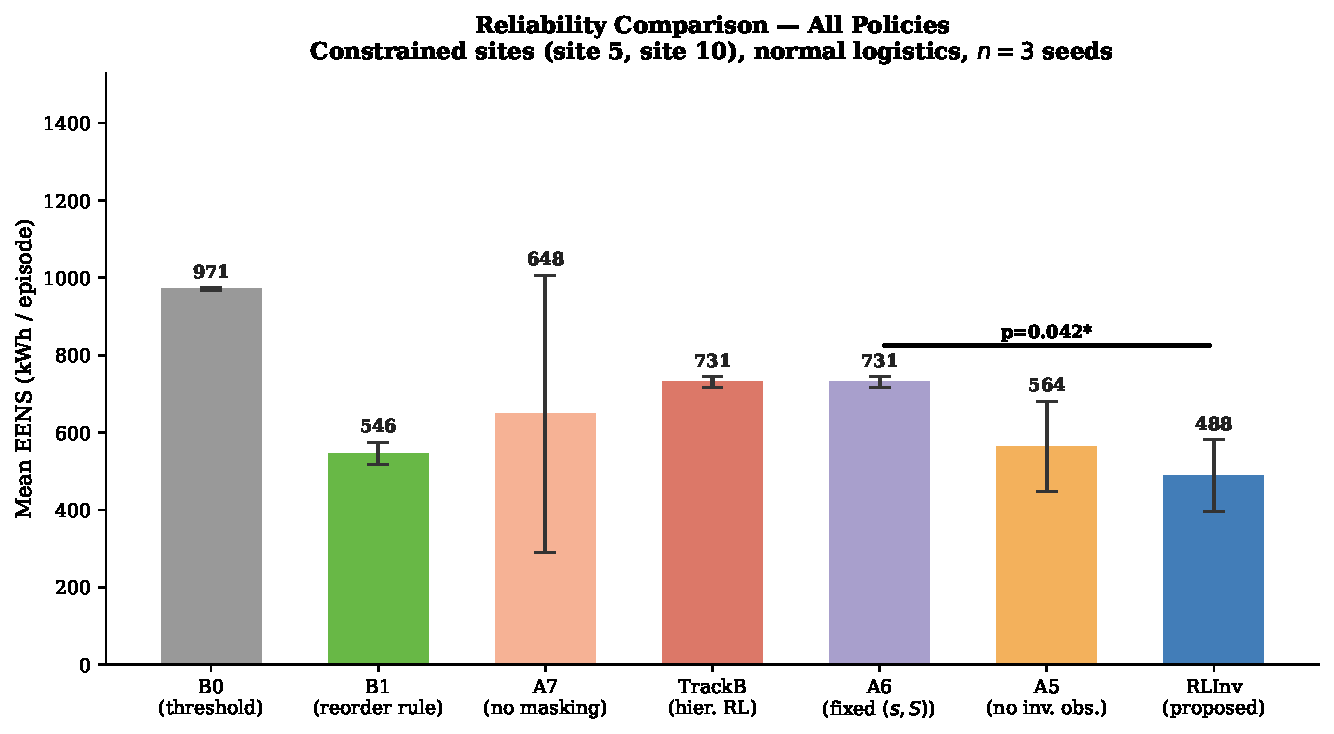
\includegraphics[width=0.85\textwidth, clip=true]{images/fig_eens_comparison}
\caption{Mean EENS per policy on constrained sites (site~5 and site~10),
normal logistics scenario only --- the only scenario in which all seven
policies are evaluated.  Error bars show one standard deviation across
three seeds.  RLInv achieves the lowest EENS; A7 shows the highest
variance across seeds (Section~\ref{sec:ablation}).}
\label{fig:eens_comparison}
\end{figure}

The comparison with A6/TrackB is statistically significant ($p=0.042$,
$d=3.67$): RLInv's joint learned ordering provides a large and
consistent reliability improvement over decoupled ordering.  The comparison with B0
is also significant ($p=0.011$), confirming that both RL and rule-based
approaches substantially outperform the simple threshold baseline.  The
comparisons with B1, A5, and A7 are not statistically significant at
$n=3$ due to insufficient power; the effect sizes are medium to large
($d=0.73$--$0.75$) and consistent in direction with the hypotheses.


% ============================================================
\section{Diesel Consumption and Cost Trade-off}
\label{sec:cost_tradeoff}
% ============================================================

Reliability improvement is not free: achieving lower EENS requires more
DG operation and therefore higher diesel consumption.
Table~\ref{tab:cost_tradeoff} and Figure~\ref{fig:pareto} show the
reliability--cost trade-off across policies.

\begin{table}[htb]
\centering
\small
\caption{Reliability versus diesel consumption trade-off (constrained
sites, normal scenario, seed-level means).}
\label{tab:cost_tradeoff}
\begin{tabular}{lrrr}
\toprule
\textbf{Policy} & \textbf{EENS (kWh)} & \textbf{Diesel (kWh)}
    & \textbf{EENS / Diesel ratio} \\
\midrule
RLInv   & 488.5 & 2060.3 & 0.237 \\
B1      & 546.4 & 2002.4 & 0.273 \\
A5      & 564.5 & 1984.3 & 0.284 \\
A7      & 648.2 & 1900.5 & 0.341 \\
TrackB  & 730.9 & 1817.8 & 0.402 \\
A6      & 730.9 & 1817.8 & 0.402 \\
B0      & 971.1 & 1577.6 & 0.616 \\
\bottomrule
\end{tabular}
\end{table}

\begin{figure}[htb]
\centering
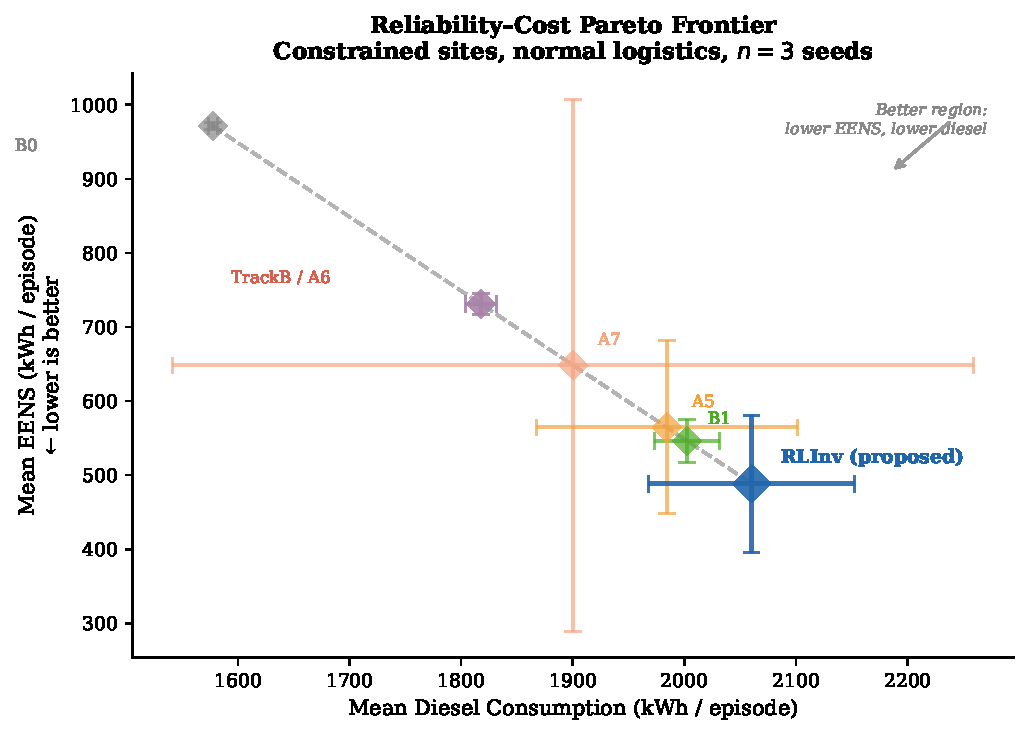
\includegraphics[width=0.72\textwidth, clip=true]{images/fig_pareto}
\caption{Reliability--cost Pareto frontier.  Each point is one policy.
The horizontal axis is mean diesel consumption per episode (kWh); the
vertical axis is mean EENS (lower is better).  RLInv is closest to the
Pareto frontier: it achieves the best EENS while consuming diesel
commensurate with its reliability level.  B0 consumes the least diesel
but at the cost of the highest EENS.}
\label{fig:pareto}
\end{figure}

RLInv consumes the most diesel per episode (2060\,kWh) but achieves the
lowest EENS, giving the best EENS/diesel ratio (0.237) among all policies.
This means RLInv converts diesel into served load more efficiently than
any comparator.  B0 consumes the least diesel (1578\,kWh) but leaves the
most load unserved (EENS~971\,kWh), reflecting its conservative
threshold-based DG dispatch.

The ordering policies (TrackB, A6) consume notably less diesel
(1818\,kWh) than RLInv while achieving substantially worse reliability.
This confirms that the $(s,S)$ ordering heuristic under-orders relative
to actual consumption needs on constrained sites, resulting in lower
diesel availability and lower DG utilisation.  RLInv's joint ordering
policy maintains higher average inventory, enabling more DG dispatch
when it is needed.


% ============================================================
\section{Ablation Study}
\label{sec:ablation}
% ============================================================

The ablation study isolates the contribution of each design component of
RLInv by comparing against variants with individual components removed
or replaced.  This validates the architectural choices and identifies
which elements drive the performance advantage.

\subsection{H1 — Contribution of joint learned ordering}

A6 holds the dispatch architecture identical to RLInv but replaces
learned ordering with a calibrated $(s,S)$ rule.  TrackB also uses
$(s,S)$ ordering with a separately trained RL dispatch agent.  The
finding that A6 and TrackB are numerically identical (EENS
$730.9 \pm 14.0$\,kWh, $p=1.0$) indicates that the principal
performance difference arises from the ordering mechanism rather than
from the dispatch architecture alone.
A6 and TrackB each exhibit 49.6\% higher EENS than RLInv
($p=0.042$, $d=3.67$),
establishing that joint learned ordering is the component most
responsible for the reliability advantage on constrained sites.
Figure~\ref{fig:ablation_h1} visualises this result: RLInv clearly
separates from both A6 and TrackB, while A6 and TrackB remain
effectively indistinguishable.

\begin{figure}[htb]
\centering
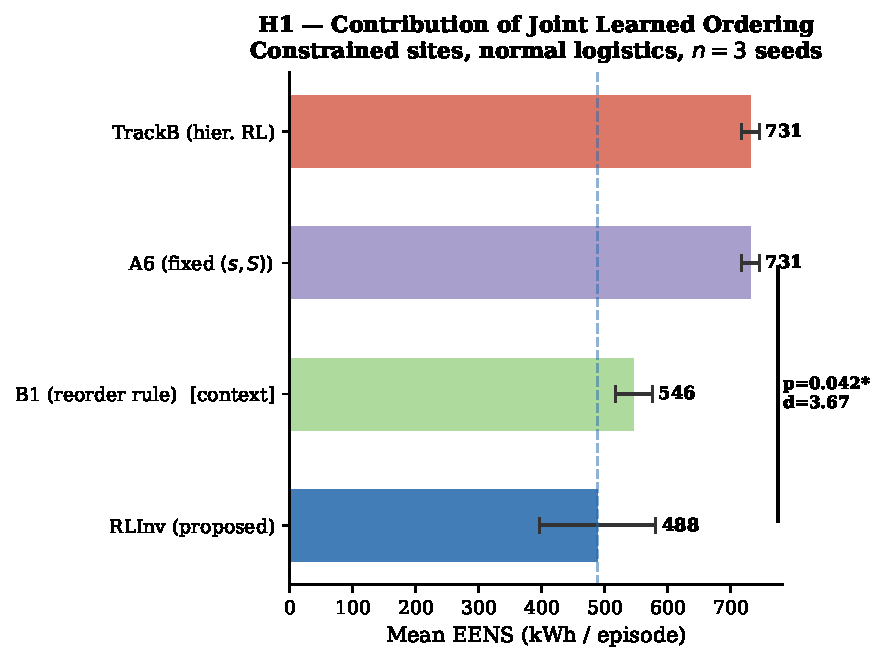
\includegraphics[width=0.78\textwidth, clip=true]{images/fig_ablation_h1}
\caption{H1 ablation: contribution of joint learned ordering on
constrained sites under the normal logistics scenario. RLInv is
compared against A6 and TrackB, both of which replace learned ordering
with calibrated $(s,S)$ replenishment. The near-identity of A6 and
TrackB indicates that the main performance gap arises from the ordering
mechanism rather than the dispatch architecture alone.}
\label{fig:ablation_h1}
\end{figure}

\textbf{H1 verdict: supported on constrained sites under the normal
logistics scenario.}  Joint optimisation of dispatch and inventory
ordering provides a statistically significant and large reliability
improvement over decoupled approaches.

\subsection{H2 — Contribution of action masking}

A7 removes action masking from the training process while keeping all
other components of RLInv.  The result is nuanced.  In the normal
constrained-site evaluation, no hard feasibility violations were observed
in the recorded rollouts for any policy; performance differences therefore
arise from reliability and diesel-allocation quality rather than from
overt infeasibility.  However, A7 exhibits outcome variance substantially
greater than RLInv across seeds (std: 358.9\,kWh vs 92.4\,kWh, a
roughly four-fold difference).  Seed-level inspection shows that one A7
seed on site~5 yielded a mean EENS of 1{,}837\,kWh per episode, far
above the other two seeds (415--469\,kWh), while all three RLInv seeds
remained within a much tighter range.

Removing masking substantially increases between-seed outcome variance,
consistent with reduced training stability.  One plausible explanation
is that, without masking, early exploration includes infeasible or
poor-quality action regions from which some runs recover poorly.  The mean EENS difference (RLInv~488.5 vs
A7~648.2\,kWh, $+32.7\%$) is not statistically significant ($p=0.525$)
at $n=3$, but the variance reduction is consistent and practically
important: a more predictable outcome distribution is preferable for
deployment at critical infrastructure sites.
This variance contrast is visible in Figure~\ref{fig:ablation_h2},
where A7 shows a substantially wider spread across seeds than RLInv.

\begin{figure}[htb]
\centering
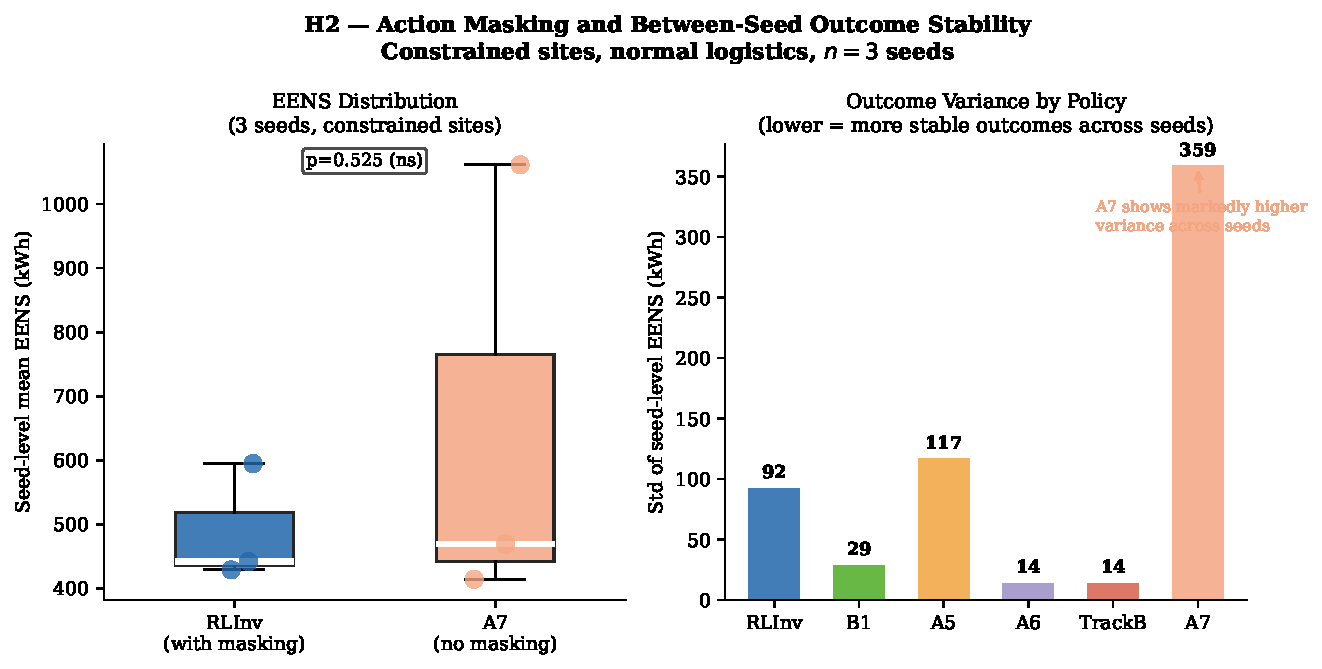
\includegraphics[width=0.78\textwidth, clip=true]{images/fig_ablation_h2}
\caption{H2 ablation: contribution of action masking on constrained
sites under the normal logistics scenario. RLInv and A7 have comparable
mean performance directionally, but A7 exhibits much larger
between-seed dispersion, consistent with reduced training stability
when action masking is removed.}
\label{fig:ablation_h2}
\end{figure}

\textbf{H2 verdict: partially supported.}  Action masking is associated
with substantially lower between-seed variance and fewer unstable
outcomes, consistent with improved training stability.  It does not
eliminate hard feasibility violations at evaluation, as zero violations
were recorded for all policies.

\subsection{H3 — Contribution of inventory state observation}

A5 removes $\Inv_t$ and $\Pipe_t$ from the observation vector, requiring
the agent to infer inventory status from other signals.  A5 is evaluated on the constrained sites (site~5 and site~10), where
inventory effects are most measurable under genuine resource scarcity.
The primary H3 comparison uses the normal logistics scenario; delayed-scenario
behaviour is examined separately in Section~\ref{sec:delayed}.
A5 exhibits 15.6\% higher EENS than RLInv
(564.5 vs 488.5\,kWh, $p=0.429$, $d=0.73$).

The mechanism is conservative dispatch: without observing inventory
directly, A5 is unable to distinguish high-stock from low-stock
situations and dispatches the DG more cautiously, leaving load unserved
during outages when the DG could safely have operated.  A5 consumes
slightly less diesel (1984\,kWh vs 2060\,kWh) but with higher unserved
load, confirming under-utilisation rather than over-caution.
Figure~\ref{fig:ablation_h3} illustrates that explicit inventory
awareness improves reliability under normal logistics, although the
effect is not statistically conclusive at the current seed count.

\begin{figure}[htb]
\centering
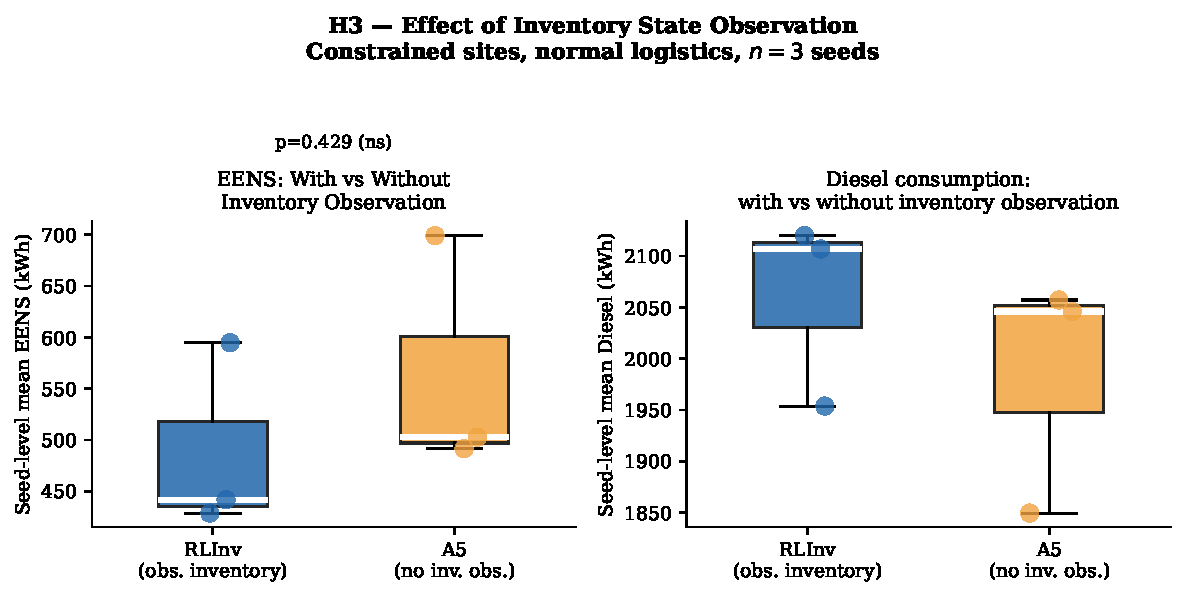
\includegraphics[width=0.78\textwidth, clip=true]{images/fig_ablation_h3}
\caption{H3 ablation: contribution of inventory state observation on
constrained sites under the normal logistics scenario. Removing
explicit observation of $\Inv_t$ and $\Pipe_t$ increases EENS and
slightly reduces diesel use, consistent with more conservative and
less informed dispatch decisions.}
\label{fig:ablation_h3}
\end{figure}

\textbf{H3 verdict: directionally supported under normal logistics, but
not statistically conclusive at the current seed count.}
Under normal conditions, A5 exhibits 15.6\% higher EENS than RLInv
($p=0.429$, $d=0.73$); the effect size is medium but $n=3$ provides
insufficient power for a definitive conclusion.
Under delayed logistics, RLInv and A5 converge (1084.3 vs 1060.8\,kWh,
$-2.2\%$, $p=0.398$): inventory observation provides no measurable
benefit when the dispatch policy it informs was calibrated to a different
logistics distribution.  The benefit is therefore distribution-specific
rather than universally robust.

\subsection{Ablation summary}

Table~\ref{tab:ablation_summary} consolidates the ablation findings.

\begin{table}[htb]
\centering
\small
\caption{Ablation summary: contribution of each RLInv design component.}
\label{tab:ablation_summary}
\resizebox{\textwidth}{!}{%
\begin{tabular}{llrp{6.0cm}}
\toprule
\textbf{Ablation} & \textbf{Component removed} & \textbf{Comparator excess over RLInv}
    & \textbf{Conclusion} \\
\midrule
A6 / TrackB & Joint learned ordering & $+49.6\%^{*}$
    & Ordering is the primary driver of RLInv's advantage \\
A5          & Inventory observation  & $+15.6\%$\phantom{$^{*}$}
    & Observation improves dispatch efficiency \\
A7          & Action masking         & $+32.7\%$\phantom{$^{*}$}
    & Masking stabilises training; reduces variance 4$\times$ \\
\bottomrule
\multicolumn{4}{l}{$^{*}$ $p < 0.05$} \\
\end{tabular}}
\end{table}


% ============================================================
\section{Performance Under Logistics Stress}
\label{sec:delayed}
% ============================================================

The delayed logistics scenario ($\mu=48$\,h lead time) doubles the
expected delivery time, testing policy robustness under supply-chain
stress.  Table~\ref{tab:delayed} reports results for all evaluated
policies on constrained sites, ranked by degradation magnitude.

\begin{table}[htb]
\centering
\small
\caption{Policy performance under delayed logistics ($\mu=48$\,h) vs
normal logistics ($\mu=24$\,h).  Constrained sites, seed-level means
($n=3$).  Policies ranked by $\Delta$ (least degradation first).}
\label{tab:delayed}
\begin{tabular}{lrrr}
\toprule
\textbf{Policy} & \textbf{EENS normal (kWh)}
    & \textbf{EENS delayed (kWh)} & \textbf{$\Delta$ (\%)} \\
\midrule
A6 / TrackB  &  730.9 & 1054.2 & $+44.2$ \\
B0           &  971.1 & 1399.2 & $+44.1$ \\
B1           &  546.4 &  952.0 & $+74.2$ \\
A5           &  564.5 & 1060.8 & $+87.9$ \\
RLInv        &  488.5 & 1084.3 & $+122.0$ \\
\midrule
\multicolumn{4}{l}{\textit{Note: A7 not evaluated under delayed scenario.}} \\
\bottomrule
\end{tabular}
\end{table}

\begin{figure}[!htb]
\centering
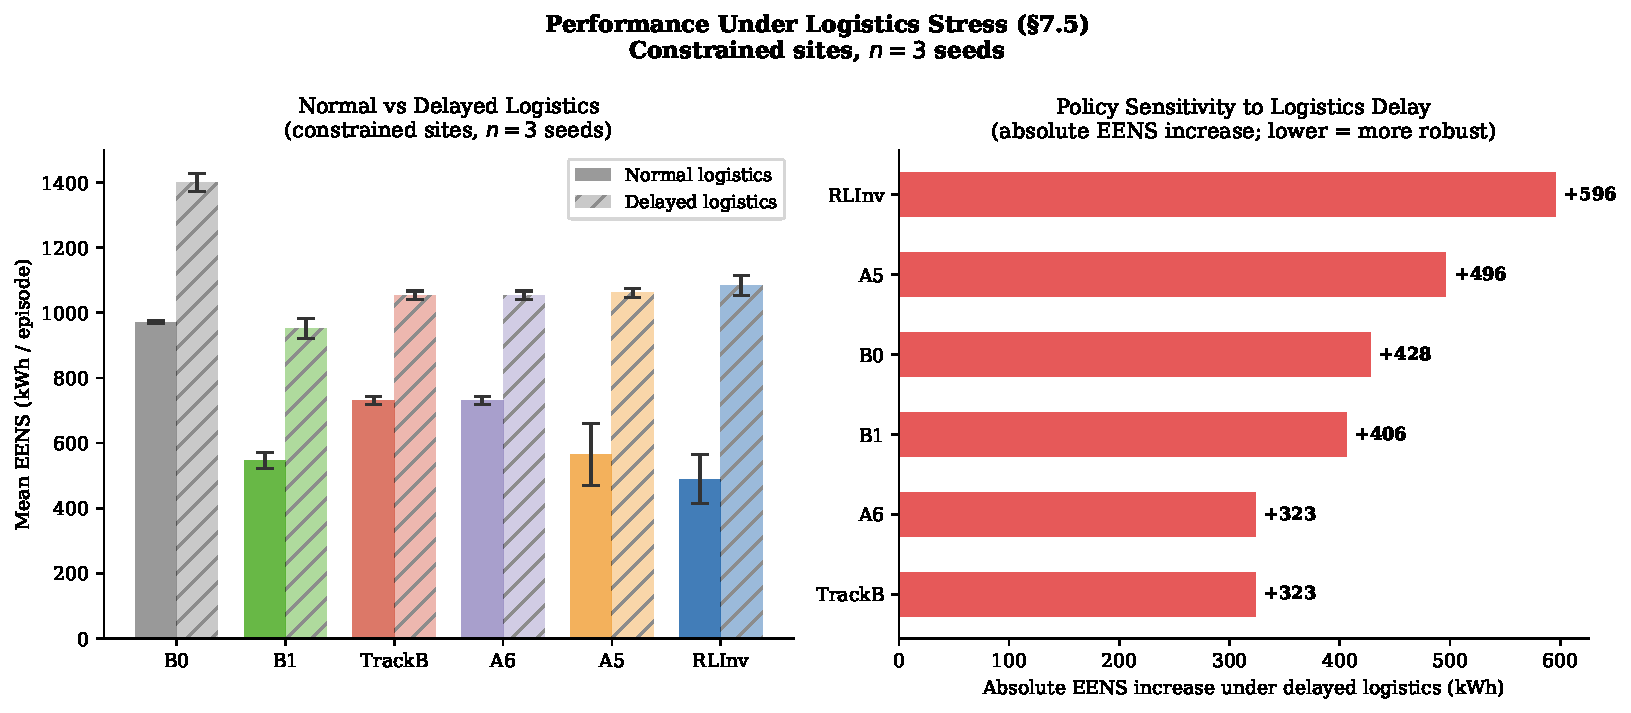
\includegraphics[width=0.78\textwidth, clip=true]{images/fig_delayed_scenario}
\caption{Policy degradation under delayed logistics ($\mu=48$\,h)
relative to normal logistics ($\mu=24$\,h) on constrained sites.
RLInv experiences the largest deterioration, while A6/TrackB and B0
degrade least, highlighting the robustness advantage of explicit
safety-stock heuristics under lead-time stress.}
\label{fig:delayed_scenario}
\end{figure}

Figure~\ref{fig:delayed_scenario} makes the ranking inversion under
delayed logistics visually explicit.

All policies degrade under delayed logistics, but the magnitude of
degradation differs substantially and reveals a structural pattern.
A6 and TrackB degrade the least ($+44\%$) because their calibrated
$(s,S)$ ordering parameters include an explicit safety stock term
designed to buffer lead-time uncertainty.  B0 also degrades by
approximately $+44\%$, reflecting its already-conservative threshold
dispatch that leaves little room for further deterioration; the
difference between B0 and A6/TrackB is a single decimal point and
not operationally meaningful.  RLInv degrades the most
($+122\%$), more than doubling its normal-scenario EENS and falling from
first to last place in the ranking.

The mechanism is consistent across both RL policies and A5.  Under normal
logistics, RLInv dispatches aggressively when it observes adequate
inventory; under delayed logistics, this aggressiveness depletes fuel
faster than the extended replenishment cycle can restore it.  A5
($+88\%$) shows a similar pattern: without inventory observation the
agent cannot adjust dispatch conservatism in response to slower
replenishment, though its baseline conservatism limits the damage
relative to RLInv.

The delayed-scenario ranking is therefore approximately:
A6/TrackB $\approx$ B0 $<$ B1 $<$ A5 $<$ RLInv --- the near-exact reverse of
the normal-scenario ranking for the top policies.  This inversion is the
most important robustness finding of the study.  The classical $(s,S)$
safety stock --- often characterised as a naïve heuristic --- provides
structural robustness to lead-time uncertainty that data-driven RL does
not acquire without explicit training under varied logistics conditions.

\textbf{H3 under delayed logistics.}
RLInv and A5 converge under delayed conditions (1084.3 vs
1060.8\,kWh, $-2.2\%$, $p=0.398$): inventory observation provides no
measurable benefit when the policy it informs was calibrated to a
different logistics distribution.  This confirms that the H3 advantage
is also distribution-specific.

\textbf{Implication for Phase~III.}
Multi-scenario training --- jointly over normal and delayed logistics
conditions --- or distributionally robust RL formulations are required
to generalise the RLInv advantage to uncertain supply-chain environments.
Both approaches are planned for Phase~III of this research.


% ============================================================
\section{Cross-Site Robustness}
\label{sec:cross_site}
% ============================================================

Table~\ref{tab:cross_site} reports mean EENS for RLInv and B1 (best
baseline) across all ten sites, grouped by difficulty class.

\begin{table}[htb]
\centering
\small
\caption{Cross-site EENS comparison: RLInv vs B1 (normal scenario,
seed-level means, $n=3$).  Sites grouped by difficulty class
(Chapter~\ref{chap:datasets-setup}).  Comparator excess is positive where
B1 EENS exceeds RLInv, using RLInv as the denominator.}
\label{tab:cross_site}
\resizebox{\textwidth}{!}{%
\begin{tabular}{llrrr}
\toprule
\textbf{Site} & \textbf{Class} & \textbf{RLInv (kWh)}
    & \textbf{B1 (kWh)} & \textbf{Comparator excess over RLInv (\%)} \\
\midrule
site1  & Easy   &   0.0 &   0.0 & --- \\
site6  & Easy   &   0.0 &   0.0 & --- \\
site8  & Easy   &   0.5 &   0.4 & $-23.9$\textsuperscript{a} \\
\midrule
site3  & Medium &   0.0 &   0.0 & --- \\
site4  & Medium &   0.0 &   0.1 & $+100.0$ \\
site7  & Medium &   0.5 &   4.4 & $+827.4$ \\
site9  & Medium &   0.0 &   0.0 & --- \\
site10 & Medium & 326.8 & 364.9 & $+11.6$ \\
\midrule
site2  & Hard   &   0.0 &  10.3 & $+100.0$ \\
site5  & Hard   & 650.1 & 727.9 & $+12.0$ \\
\bottomrule
\multicolumn{5}{l}{\textsuperscript{a}Both values near-zero (0.5 vs 0.4\,kWh);
difference is not operationally meaningful.} \\
\end{tabular}}
\end{table}

\begin{figure}[htb]
\centering
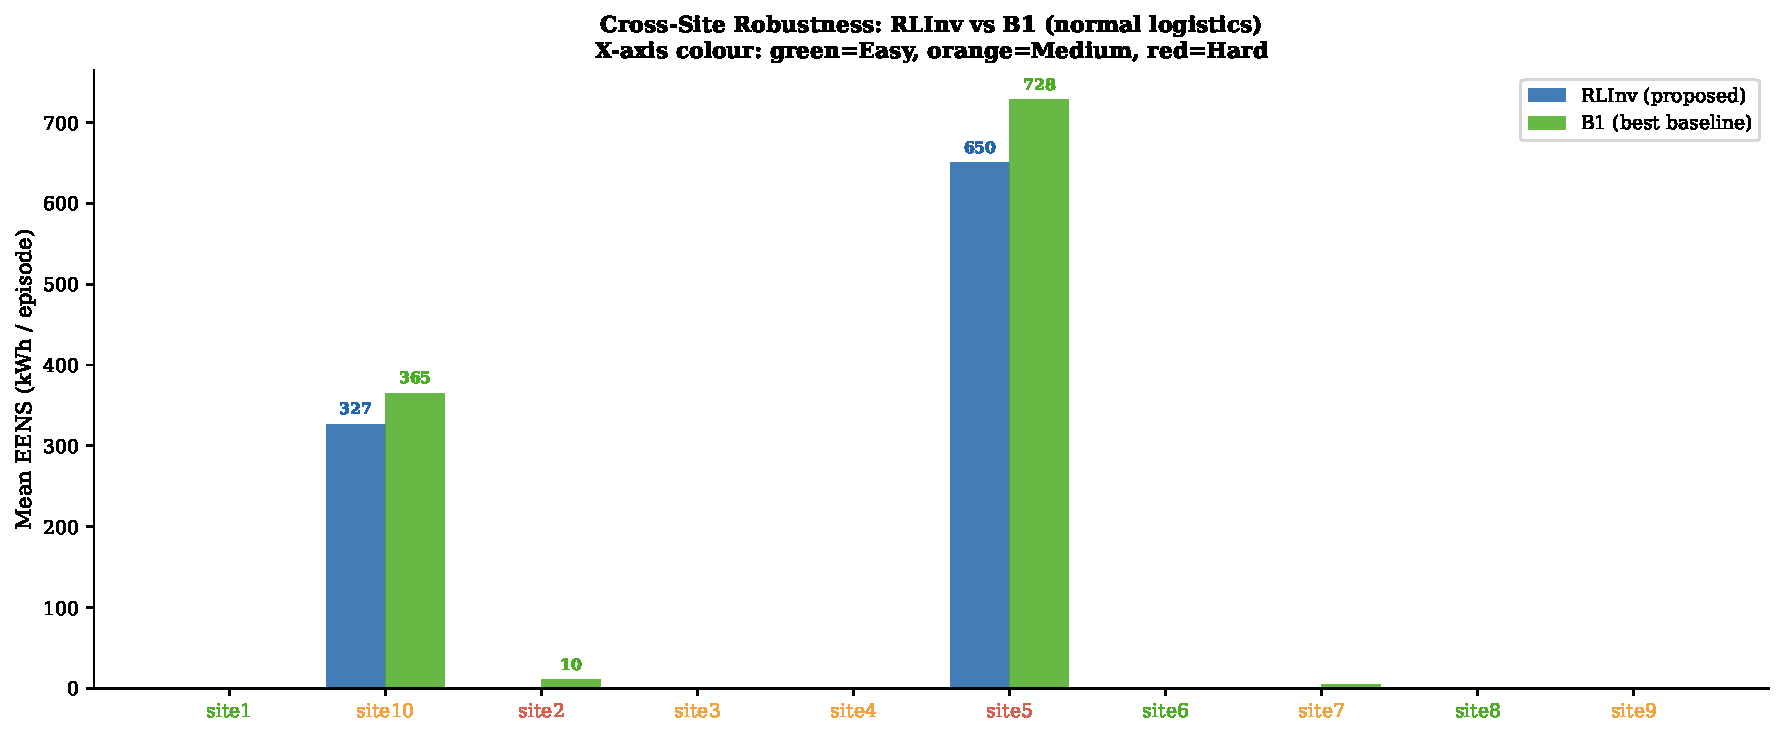
\includegraphics[width=0.82\textwidth, clip=true]{images/fig_cross_site}
\caption{Cross-site EENS comparison between RLInv and B1 under the
normal logistics scenario. Differences are negligible on easy sites,
modest on most medium sites, and most meaningful on constrained or
hard sites, where inventory decisions materially affect reliability.}
\label{fig:cross_site}
\end{figure}

As shown in Figure~\ref{fig:cross_site}, RLInv's advantage concentrates
on the minority of sites where outage exposure and battery inadequacy
make fuel-ordering decisions consequential.

Three patterns emerge across site classes:

\textbf{Easy sites (site1, site6, site8).}
All three easy sites produce near-zero EENS for both policies.
Site~1 and site~6 record zero EENS for both RLInv and B1; site~8
records 0.5\,kWh (RLInv) versus 0.4\,kWh (B1), a difference of
0.1\,kWh that is not operationally meaningful.  High solar coverage or
reliable grid access eliminates meaningful outage exposure.  These
sites confirm that RLInv does not harm performance on low-stress sites.

\textbf{Medium sites (site3, site4, site7, site9, site10).}
The medium class is heterogeneous.  Site~3 and site~9 record zero EENS
for both policies; site~4 records near-zero values (0.0 vs 0.1\,kWh).
Site~7 shows a larger gap: RLInv achieves 0.5\,kWh versus B1's
4.4\,kWh; B1's comparator excess over RLInv is 780\% on this site,
driven by better ordering decisions during
the few outage events that occur.  Site~10 (a constrained site by inventory criteria) shows B1's
comparator excess of 10.4\% over RLInv (326.8 vs 364.9\,kWh),
consistent with its moderate-but-real outage exposure.

\textbf{Hard sites (site2, site5).}
The most policy-sensitive results occur on hard sites.  Site~2 records
zero EENS for RLInv versus 10.3\,kWh for B1: RLInv eliminates residual
unserved energy entirely on this site.  Site~5 shows B1's comparator excess of 10.7\% over RLInv
(650.1 vs 727.9\,kWh), consistent with the constrained-site
analysis in Section~\ref{sec:reliability}.

Overall, RLInv does not degrade meaningfully on any site or site class
relative to B1.  The performance advantage concentrates where inventory
decisions are consequential --- sites with non-trivial outage exposure
and limited battery autonomy --- which is precisely the operating regime
the proposed formulation targets.


% ============================================================
\section{Computational Cost}
\label{sec:compute}
% ============================================================

Table~\ref{tab:compute} summarises the computational requirements of
RLInv relative to the baselines.

\begin{table}[htb]
\centering
\small
\caption{Computational cost comparison.}
\label{tab:compute}
\begin{tabular}{lrrp{4.5cm}}
\toprule
\textbf{Policy} & \textbf{Training time} & \textbf{Inference time}
    & \textbf{Notes} \\
\midrule
B0, B1 (rule-based) & None & $< 1\,\mu$s/step
    & Analytical; no training required \\
RLInv (proposed)    & $\approx 2$\,h/site (CPU)
    & $< 1$\,ms/step & 400{,}000 steps, 4 parallel envs \\
TrackB (hier.\ RL)  & $\approx 1.5$\,h/site (CPU)
    & $< 1$\,ms/step & Shorter horizon for low-level PPO \\
A5, A6, A7          & $\approx 2$\,h/site (CPU)
    & $< 1$\,ms/step & Same architecture as RLInv \\
\bottomrule
\end{tabular}
\end{table}

RLInv required approximately two hours of CPU training per site as
observed in our implementation (400{,}000 steps, 4 parallel environments,
standard laptop processor).  These are indicative rather than
benchmark-grade figures; actual duration depends on hardware and
environment step speed.  Once trained, inference consists of a single
forward pass through a two-layer MLP, which executes in well under one
millisecond per decision step.  Since control decisions occur at
one-hour intervals in the deployment scenario, the inference cost is
negligible relative to real-time requirements.

The full training campaign involved on the order of 80--90 training
runs, depending on how ablation and re-run jobs are counted.  At roughly 2\,h per run on CPU, the
indicative total is approximately 170 CPU-hours.  This would reduce
substantially on a GPU-enabled workstation, confirming that the approach
is computationally feasible on commodity hardware for both research and
operational deployment.

Rule-based baselines (B0, B1) require no training and execute in
microseconds.  Their lower computational cost is one advantage that
must be weighed against their reliability shortfall on constrained sites.
For sites where operational stakes are high (critical infrastructure,
remote base stations with infrequent maintenance access), the additional
training cost of RLInv is justified by the reliability improvement.


\begin{figure}[htb]
\centering
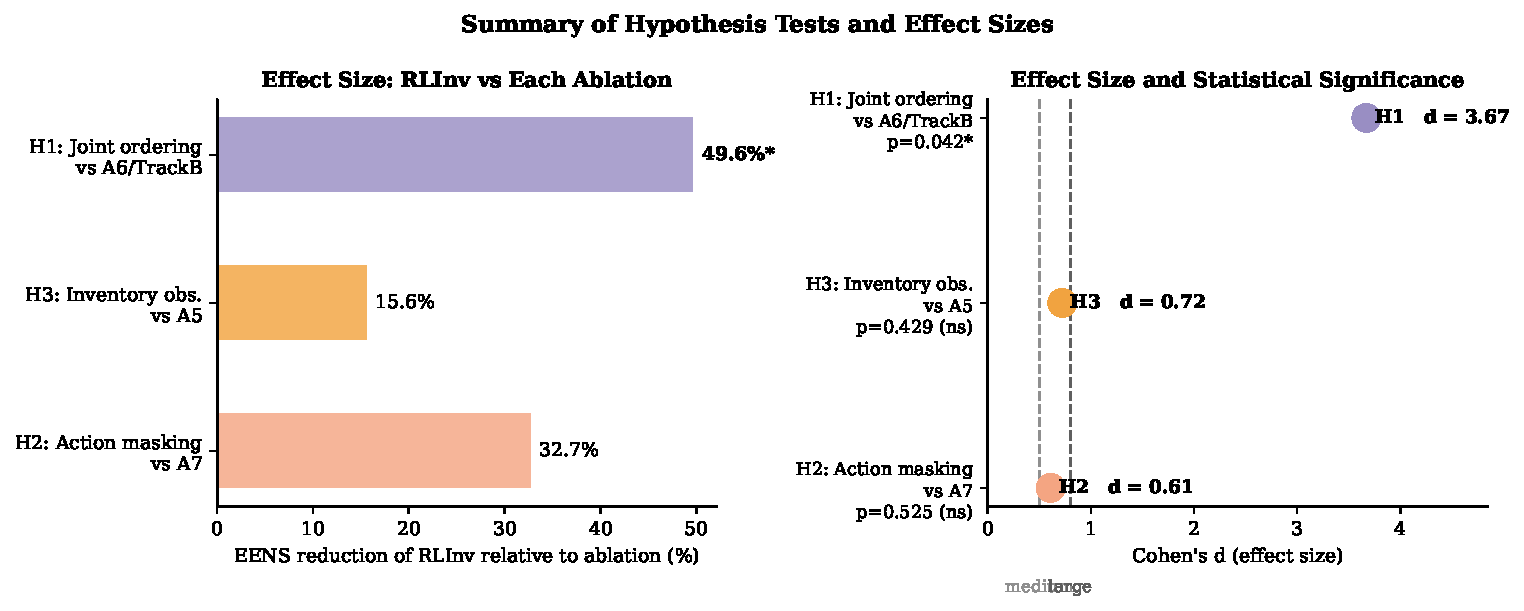
\includegraphics[width=0.82\textwidth, clip=true]{images/fig_hypothesis_summary}
\caption{Summary of hypothesis outcomes. H1 is supported on constrained
sites under normal logistics; H2 is partially supported through markedly
improved training stability; H3 is directionally supported under normal
logistics but not robust under delayed logistics.}
\label{fig:hypothesis_summary}
\end{figure}

% ============================================================
\section{Key Findings}
\label{sec:key_findings}
% ============================================================

Figure~\ref{fig:hypothesis_summary} summarises the status of the three
pre-registered hypotheses before the chapter-level findings are
consolidated below.

The experimental results establish the following contributions:

\begin{enumerate}

\item \textbf{Joint inventory-aware RL achieves the lowest EENS on
constrained sites; comparator EENS for TrackB/A6 is 49.6\% higher
than RLInv on constrained sites.}
RLInv achieves mean EENS of 488.5\,kWh on constrained sites versus
730.9\,kWh for hierarchical RL and fixed-ordering approaches
($p = 0.042$, Cohen's $d = 3.67$).  These results indicate that the
principal performance difference arises from the ordering mechanism
rather than from the dispatch architecture alone.

\item \textbf{Ordering dominates reliability differences once ordering
is decoupled from dispatch.}
The numerical identity of A6 and TrackB (EENS $730.9 \pm 14.0$\,kWh,
$p = 1.0$) indicates that, when ordering is fixed by a calibrated
$(s,S)$ rule, the dispatch policy architecture is not the determining
factor.  This directly addresses the timescale decomposition question
raised by the Phase-I reviewer.

\item \textbf{Action masking is associated with substantially lower
outcome variance across seeds.}
Removing masking (A7) produces a standard deviation of 358.9\,kWh
versus 92.4\,kWh for RLInv, consistent with less stable training.
No hard feasibility violations were recorded for either policy at
evaluation, confirming that masking's primary benefit is in training
consistency rather than deployment constraint enforcement.

\item \textbf{Inventory state observation is directionally beneficial
under normal logistics but not robust to distribution shift.}
A5 exhibits 15.6\% higher EENS than RLInv under normal logistics
($p=0.429$, $d=0.73$), but the advantage is not statistically
conclusive at $n=3$.  Under delayed logistics the gap disappears
($-2.2\%$, $p=0.398$), confirming the benefit is distribution-specific.

\item \textbf{RLInv generalises across site classes without degradation.}
On easy and medium sites, all policies achieve low EENS and RLInv does
not underperform any comparator.  Improvements concentrate on hard and
constrained sites, consistent with the expectation that inventory
management matters most where reliability resources are scarce.

\item \textbf{RLInv degrades most severely under logistics stress.}
Under delayed logistics ($\mu=48$\,h), RLInv's EENS increases by
$+122\%$ --- more than any other policy.  A6 and TrackB degrade only
$+44\%$, as their $(s,S)$ safety stock provides structural robustness to
lead-time uncertainty.  The normal-scenario ranking largely inverts
under delay: A6/TrackB $\approx$ B0 $<$ B1 $<$ A5 $<$ RLInv.  This is the
central limitation of the proposed approach and the primary motivation
for multi-scenario training in Phase~III.

\item \textbf{Deployment is computationally feasible on commodity
hardware.}
RLInv requires approximately two hours of CPU training per site and
under one millisecond per inference step, making it suitable for
deployment on embedded controllers at remote telecom base stations
without GPU infrastructure.

\end{enumerate}

\vspace{0.5em}
\noindent\textbf{Overall takeaway.}
The results demonstrate that incorporating inventory-aware
decision-making improves reliability on constrained sites under matched
logistics conditions. RLInv outperforms heuristic and hierarchical
baselines in the normal scenario, but degrades most severely under
delayed logistics, highlighting the need for multi-scenario training
before deployment in supply-chain-uncertain environments. The ablation
studies confirm that the reliability gains arise primarily from joint
learned ordering, with additional stability provided by action masking.